

\section{Multiple Regression in R}

To illustrate multiple regression in R we'll use a built in dataset called |trees|. |trees| consists of measurements of the girth, height, and volume of 31 black cherry trees (|?trees| for more info). We'll start with some summary tables and diagnostic plots to familiarize ourselves with the data:
%
\begin{R}
> names(trees)
[1] "Girth"  "Height" "Volume"
> dim(trees)
[1] 31  3
> summary(trees)
     Girth           Height       Volume
 Min.   : 8.30   Min.   :63   Min.   :10.20
 1st Qu.:11.05   1st Qu.:72   1st Qu.:19.40
 Median :12.90   Median :76   Median :24.20
 Mean   :13.25   Mean   :76   Mean   :30.17
 3rd Qu.:15.25   3rd Qu.:80   3rd Qu.:37.30
 Max.   :20.60   Max.   :87   Max.   :77.00
> library(PerformanceAnalytics)
> chart.Correlation(trees)
\end{R}
%
As one might expect, the scatterplot matrix shows that all the variables are positively correlated, and girth and volume have a  particularly strong correlation.

Let's assume we're lumberjacks, but our permit only allows us to harvest a fixed number of trees.  We get paid by the total volume of wood we harvest, so we're interested in predicting a tree's volume (hard to measure directly) as a function of its girth and height (relatively easy to measure), so we can pick the best trees to harvest.  We'll therefore calculate a multiple regression of volume on height and width. Let's start by taking a look at the 3D scatter of the data using the plot3d function from the |rgl| package.
%
\begin{R}
> library(rgl)
> plot3d(trees, col='red', size=1, type='s') # use your mouse to rotate the plot
\end{R}
%
From the 3D scatter plot it looks like we ought to be able to find a plane through the data that fits the scatter fairly well. Let's use the |lm()| function to calculate the multiple regression:
%
\begin{R}
> l <- lm(Volume ~ Girth + Height, data=trees)
\end{R}
%
To visualize the multiple regression, let's use the |scatterplot3d| package to draw the 3D scatter of plots and the plane that corresponds to the regression model:
%
\begin{R}
> p <- scatterplot3d(trees,angle=55,type='h')
> title('Tree Volume as\na function of Girth and Height')
> p$plane3d(l, col='orangered')  # dark pink color
> dev.copy(pdf, 'trees-regrfit.pdf')  # copy plot to a pdf file
> dev.off()  # write the file
\end{R}
%
Notice the use of |dev.copy()| and |dev.off()| to save the plot from the console.  The output this generates should look similar to Fig.~\ref{fig:treesregr}.
%
\begin{figure}[htbp]
\centering
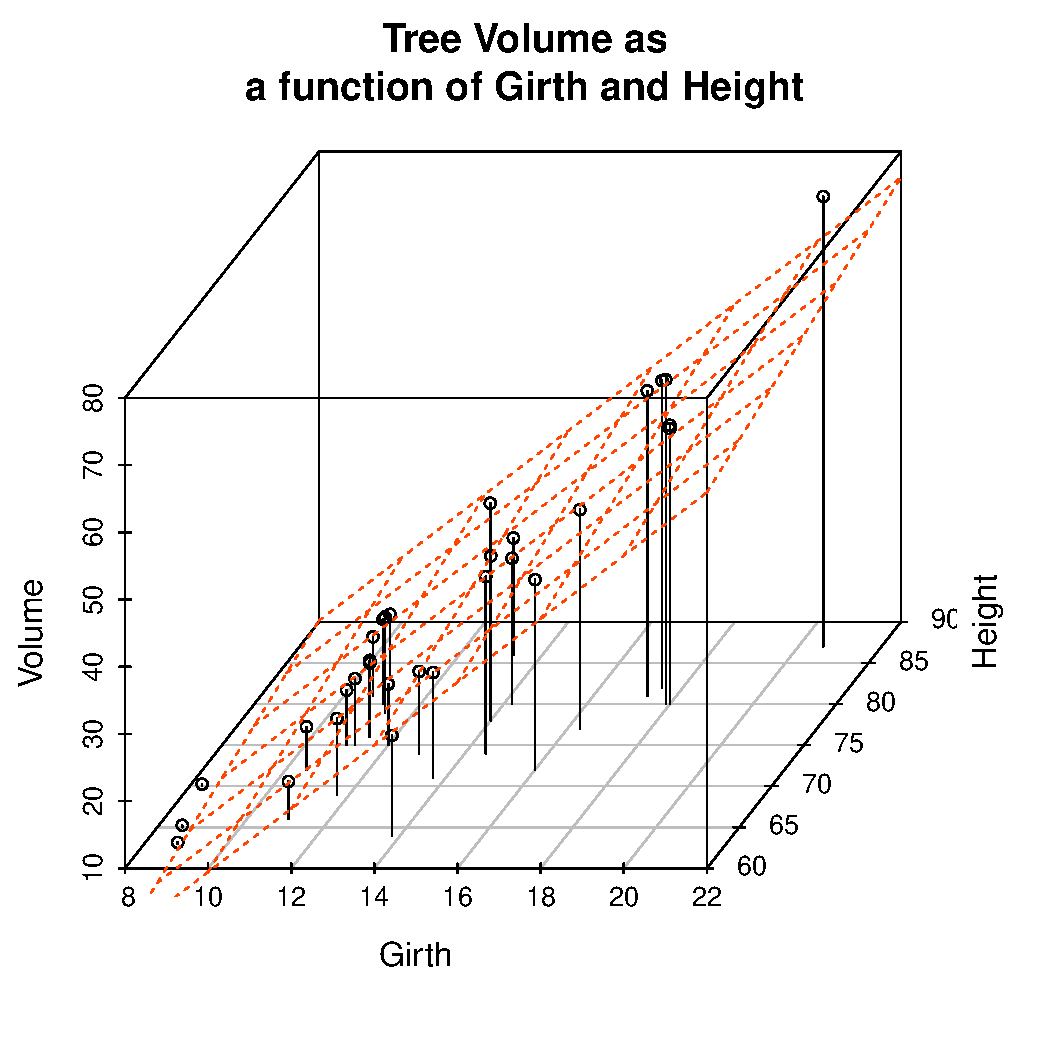
\includegraphics[width=0.5\columnwidth]{./figures/hands-on4/trees-regrfit.pdf}
\caption{Multiple regression plot of cherry tree volume on girth and height, generated using the \texttt{scatterplot3d} library\label{fig:treesregr}}
\end{figure}

From the figure it looks like the regression model fits pretty well (we could have anticipated that from the pairwise relationships).  Let's use the |summary()| function to obtain details of the fit:
\begin{R}
> summary(l)

Call:
lm(formula = Volume ~ Girth + Height, data = trees)

Residuals:
    Min      1Q  Median      3Q     Max
-6.4065 -2.6493 -0.2876  2.2003  8.4847

Coefficients:
            Estimate Std. Error t value Pr(>|t|)
(Intercept) -57.9877     8.6382  -6.713 2.75e-07 ***
Girth         4.7082     0.2643  17.816  < 2e-16 ***
Height        0.3393     0.1302   2.607   0.0145 *
---
Signif. codes:  0 ‘***’ 0.001 ‘**’ 0.01 ‘*’ 0.05 ‘.’ 0.1 ‘ ’ 1

Residual standard error: 3.882 on 28 degrees of freedom
Multiple R-squared: 0.948,  Adjusted R-squared: 0.9442
F-statistic:   255 on 2 and 28 DF,  p-value: < 2.2e-16
\end{R}
%
We see that the coefficients for both Girth and Height are significant at the $p<0.05$ level, but that Girth is the much stronger predictor. In fact the addition of height explains only a minor additional fraction of variation in tree volume, so from the lumberjack's perspective the additional trouble of measuring height probably isn't worth it.

The object returned by the |lm()| function hold lots of useful information:
%
\begin{R}
> names(l)
 [1] "coefficients"  "residuals"     "effects"       "rank"          "fitted.values" "assign"
 [7] "qr"            "df.residual"   "xlevels"       "call"          "terms"         "model"
\end{R}
%
Let's look at the residuals from the regression. The residuals represent the `unexplained' variance:
\begin{R}
> plot(trees$Volume,l$residuals, xlab='Volume',ylab='Regression Residuals')
> abline(h=0, lty='dashed', col='red')
\end{R}
%
Ideally the residuals should be evenly scatter around zero, with no trends as we go from high to low values of the outcome value.  As you can see in Fig.~\ref{fig:trees-resid} it looks like that the residuals on the left tend to be below zero, while those on the far right of the plot are consistently above zero, suggesting that there may be a non-linear aspect of the relationship that our model isn't capturing.
%
\begin{figure}[htbp]
\centering
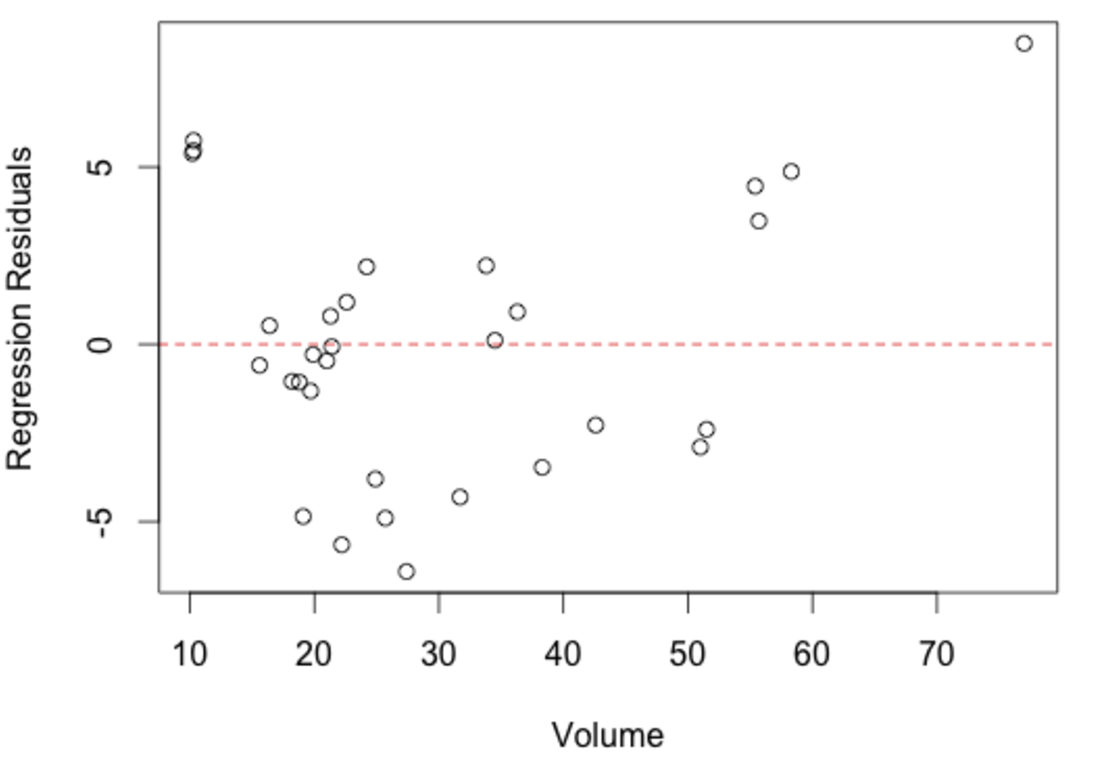
\includegraphics[width=0.65\columnwidth]{./figures/hands-on4/trees-residuals.pdf}
\caption{Residual plot based on the multiple regression plot of cherry tree volume on girth and height,\label{fig:trees-resid}}
\end{figure}


% This weeks hands-on exercises draw from a nice set of introductory R
% notes written by John Verzani, entitled ``simpleR -- Using R for
% Introductory Statistics.'' This text used to available online at:
% \url{http://www.math.csi.cuny.edu/Statistics/R/simpleR/} (the page still
% exists, but the PDF is not available as of Sept. 2011, but see below). I've put up a
% \href{https://raw.github.com/pmagwene/Bio313/master/lecture-04/simpleR.pdf}{PDF version of the Verzani text} on GitHub. Also from the class wiki
% download the set of R functions and data that are associated with the
% Verzani text
% \href{https://raw.github.com/pmagwene/Bio313/master/lecture-04/simpleR.R}{\lstinline!simpleR.R!}
% and put it in your R working directory.

% \section{Bivariate Linear Regression in R revisited}

% Recall from previous class sessions that the main function for carrying
% out regression in R is \lstinline!lm()! (short for linear-model). Read and work through the exercises in Verzani, section 13 (starting at
% p.~100 in the PDF), for a refresher on bivariate regression. As you work
% through the material you will notice that Verzani uses a number of
% functions that are defined in the code file \lstinline!simple.R!, for
% example \lstinline!simple.lm()!. Most of these are what me might call
% ``wrapper functions'' --- they wrap pre-existing R functions to make
% them more convenient to use, for example automatically creating useful
% plots.


% \end{assignment}

% \section{Multiple Regression in R}

% Like bivariate regression, multiple regression in R is typically
% conducted using the \lstinline!lm()! function. Work through Verzani
% section 14 (p.~109 in the PDF). On p.~114 Verzani demonstrates an
% application of polynomial regression.

% \section{Logistic Regression in R}

% Logistic regression is a type of `Generalized Linear Model' (GLM) and
% hence is fit using the \lstinline!glm()! function in R.
% \lstinline!glm()! can also be used to fit other types of generalized
% linear models so one must specify the model type as shown below. We will
% apply logistic regression to study natural selection on a population of
% house sparrows.

% \subsection{Bumpus' Sparrow Data}

% Bumpus (1898) described a sample of house sparrows which he collected
% after a very severe storm. The sample included 136 birds, sixty four of
% which perished during the storm. Also included in his description were a
% variety of morphological measurements on the birds and information about
% their sex and age (for male birds). This data set has become a benchmark
% in the evolutionary biology literature for demonstrating methods for
% analyzing natural selection. The bumpus data set is available from the
% class website as \lstinline!bumpus-data.txt!.

% Bumpus, H. C. 1898. The elimination of the unfit as illustrated by the
% introduced sparrow, Passer domesticus. (A fourth contribution to the
% study of variation.) \emph{Biol. Lectures: Woods Hole Marine Biological
% Laboratory}, 209--225.

% \subsection{Using logistic regression to analyze the Bumpus data}

% We'll load the Bumpus data set and rename the variable names to shorter,
% more convenient ones.

% \begin{R}
% > bumpus <- read.delim("bumpus-data.txt")
% > names(bumpus)
%  [1] "line.number"                 "sex"                         "age..a...adult..y...young."
%  [4] "survived"                    "total.length..mm."           "alar.extent..mm."
%  [7] "weight..g."                  "length.of.beak.and.head"     "length.of.humerus..in."
% [10] "length.of.femur..in."        "length.of.tibiotarsus..in."  "width.of.skull..in."
% [13] "length.of.sternal.keel..in."
% > split.names <- strsplit(names(bumpus), ".", fixed=T)
% > split.names[1]
% [[1]]
% [1] "line"   "number"
% > split.names[8]
% [[1]]
% [1] "length" "of"     "beak"   "and"    "head"
% > first <- function(x){x[1]}
% > third <- function(x){x[3]}
% > new.names1 <- unlist(lapply(g[1:7],first))
% > new.names2 <- unlist(lapply(g[8:13],third))
% > new.names <- c(new.names1, new.names2)
% > new.names
%  [1] "line"        "sex"         "age"         "survived"    "total"       "alar"
%  [7] "weight"      "beak"        "humerus"     "femur"       "tibiotarsus" "skull"
% [13] "sternal"
% > names(bumpus) <- new.names
% \end{R}
% Having made the names more convenient we can now proceed to carrying out
% the logistic regression:

% \begin{R}
% > weight <- bumpus$weight
% > survived <- bumpus$survived
% > plot(survived ~ weight)
% > fit <- glm(formula = survived ~ weight, family=binomial(link=logit))
% > summary(fit)

% Call:
% glm(formula = survived ~ weight, family = binomial(link = logit))

% Deviance Residuals:
%     Min       1Q   Median       3Q      Max
% -1.6331  -1.1654   0.8579   1.0791   1.4626

% Coefficients:
%             Estimate Std. Error z value Pr(>|z|)
% (Intercept)   8.0456     3.2516   2.474   0.0133 *
% weight       -0.3105     0.1272  -2.441   0.0146 *
% ---
% Signif. codes:  0 '***' 0.001 '**' 0.01 '*' 0.05 '.' 0.1 ' ' 1

% (Dispersion parameter for binomial family taken to be 1)

%     Null deviance: 188.07  on 135  degrees of freedom
% Residual deviance: 181.58  on 134  degrees of freedom
% AIC: 185.58

% Number of Fisher Scoring iterations: 4
% > newx <- seq(20,35,0.5)
% > p <- predict.glm(fit, newdata=data.frame(weight = newx), type="response")
% > lines(newx,p)
% \end{R}

% \medskip
% \begin{assignment}
% Repeat the logistic regression of survival as a
% function of body weight for: 1)the female birds and 2) the adult male
% birds. Produce plots illustrating these regressions for each sex.
% \end{assignment}

% \subsection{LOESS Models}

% LOESS (aka LOWESS; `Locally weighted scatterplot smoothing') is a
% modeling technique that fits a curve (or surface) to a set of data using
% a large number of local regressions. Local weighted regressions are fit
% at numerous regions across the data range, using a weighting function
% that drops off as you move away from the center of the fitting region
% (hence the `local' aspect). LOESS combines the simplicity of least
% squares fitting with the flexibility of non-linear techniques and
% doesn't require the user to specify a functional form ahead of time in
% order to fit the model. It does however require relatively dense
% sampling in order to produce robust fits.

% Formally, at each point $x_i$ we estimate the regression coefficients
% $\hat{\beta}_j(x)$ as the values that minimize:
% \[\sum_{k=1}^n w_k(x_i)(y_k - \beta_0 - \beta_1 x_k - \ldots - \beta_d x_k^2)^2\]
% where $d$ is the degree of the polynomial (usually 1 or 2) and $w_k$ is
% a weight function. The most common choice of weighting function is
% called the ``tri-cube'' function which is defined as:

% \lstDeleteShortInline|
% \begin{align*}
%  w(x) & = (1-|x|^3)^3, \mbox{for}\ |x| < 1  \\
%       & = 0,\ \mbox{for}\ |x| \geq 1
% \end{align*}
% \lstMakeShortInline|


% \medskip
% \begin{assignment}
% Write an R function that computes the tri-cube
% function described above. Create a plot of the tri-cube function over
% the range (--3,3). Create a second R function that calculates the
% Gaussian function $f(x) = e^{-x^2}$ and plot that function over the same
% range in the same plot. If you're struggling with writing the functions
% you may wish to review Chapter 6 of Paradis, R for Beginners (see wiki)
% and Chapters 9 (Grouping, loops and conditional execution) and 10
% (Writing your own functions) in the ``R Introduction'' included with R.
% \end{assignment}

% The primary parameter that a user must decide on when using LOESS is the
% size of the neighborhood function to apply (i.e.~over what distance
% should the weight function drop to zero). This is referred to as the
% ``span'' in the R documentation, or as the parameter $\alpha$ in many of
% the papers that discuss LOESS. The appropriate span can be determined by
% experimentation or, more rigorously by cross-validation.

% We'll illustrate fitting a Loess model using data on Barack Obama's
% approval ratings over the period from November 2008 to September 2010
% (\lstinline!obama-polls.txt! available on the class wiki).

% \begin{R}
% > polls <- read.table('obama-polls.txt',header=T,sep="\t")
% > names(polls)
% [1] "Pollster"   "Dates"      "N.Pop"      "Approve"    "Disapprove" "Undecided"
% > dim(polls)
% [1] 854   6
% # polls in reverse chronological order so let's reverse them
% # so we can look at trend from earliest to most recent dates
% > approve <- rev(polls$Approve)
% > pollnum <- 1:length(approve)
% > loess.app <- loess(approve ~ pollnum)
% > pred.app <- predict(loess.app, pollnum)

% # illustrate Loess with a smaller neighborhood span
% > loess.app2 <- loess(approve ~ pollnum, span=0.25)
% > pred.app2 <- predict(loess.app2, pollnum)
% > lines(pollnum, pred.app2, lwd=2, col='cyan')
% \end{R}
% Take note of how the loess curve changed when we made the span smaller.
% By decreasing the span we've increased the sensitivity of the model
% (perhaps overfitting in this case).

% \medskip
% \begin{assignment}
% Write an R function that genereates a plot that
% simultaneously illustrates trends in both approval and disapproval
% ratings for Barack Obama, showing both the raw data and corresponding
% loess fits. Use colors and/or shapes to distinguish the two trends. Make
% sure both your x- and y-axes are scaled to show the full range of the
% data. Label your axes and create a title in the plot. Aim for a
% `publication quality' figure.
% \end{assignment}


